\documentclass[11pt]{article}
\newcommand{\MODULETAG}{Module 5\,\textbar\,Grade Estimation}
% ===== Toro Resource Estimation Course - shared PDF preamble =====
\usepackage[a4paper,margin=2.4cm,headsep=14pt]{geometry}
\usepackage{amsmath,amssymb}
\usepackage{lmodern}
\usepackage[T1]{fontenc}
\usepackage[utf8]{inputenc}
\usepackage{microtype}
\usepackage{graphicx}
\usepackage{booktabs}
\usepackage{array}
\usepackage{enumitem}
\usepackage{xcolor}
\usepackage{titlesec}
\usepackage{fancyhdr}
\usepackage[most]{tcolorbox}
\usepackage{listings}
\usepackage{caption}
\usepackage[hidelinks]{hyperref}

% ---- palette ----
\definecolor{navy}{HTML}{1F2A44}
\definecolor{navy2}{HTML}{2B3A5C}
\definecolor{bronze}{HTML}{C8702D}
\definecolor{bronzed}{HTML}{A85A1F}
\definecolor{teal}{HTML}{2A7D8C}
\definecolor{tealw}{HTML}{ECF4F5}
\definecolor{ink}{HTML}{26303F}
\definecolor{paper2}{HTML}{F3EDE1}
\definecolor{line}{HTML}{D8D4CB}
\definecolor{codebg}{HTML}{1C2433}
\definecolor{good}{HTML}{3F7D5A}
\definecolor{warn}{HTML}{B4451F}

\color{ink}
\setlength{\parindent}{0pt}
\setlength{\parskip}{6pt}
\linespread{1.06}

% ---- section styling ----
\titleformat{\section}{\Large\bfseries\color{navy}}{\thesection}{0.6em}{}
\titleformat{\subsection}{\large\bfseries\color{navy2}}{\thesubsection}{0.6em}{}
\titleformat{\subsubsection}{\normalsize\bfseries\color{bronzed}}{}{0em}{}
\titlespacing{\section}{0pt}{16pt}{6pt}
\titlespacing{\subsection}{0pt}{12pt}{4pt}

% ---- header / footer ----
\pagestyle{fancy}
\fancyhf{}
\renewcommand{\headrulewidth}{0.4pt}
\renewcommand{\footrulewidth}{0pt}
\fancyhead[L]{\footnotesize\color{navy2}\MODULETAG}
\fancyhead[R]{\footnotesize\color{navy2}Toro Tin Project\,\textbar\,ANRML26-137}
\fancyfoot[C]{\footnotesize\color{navy2}\thepage}

% ---- callout boxes ----
\newtcolorbox{keybox}[1][Key concept]{breakable,enhanced,
  colback=paper2,colframe=bronze,boxrule=0pt,leftrule=4pt,
  arc=2pt,left=10pt,right=10pt,top=8pt,bottom=8pt,
  fonttitle=\bfseries\sffamily\small\color{bronzed},title={#1}}
\newtcolorbox{torobox}[1][Toro application]{breakable,enhanced,
  colback=navy!6,colframe=navy,boxrule=0pt,leftrule=4pt,
  arc=2pt,left=10pt,right=10pt,top=8pt,bottom=8pt,
  fonttitle=\bfseries\sffamily\small\color{navy},title={#1}}
\newtcolorbox{pitbox}[1][Common pitfall]{breakable,enhanced,
  colback=warn!7,colframe=warn,boxrule=0pt,leftrule=4pt,
  arc=2pt,left=10pt,right=10pt,top=8pt,bottom=8pt,
  fonttitle=\bfseries\sffamily\small\color{warn},title={#1}}
\newtcolorbox{notebox}[1][Note]{breakable,enhanced,
  colback=tealw,colframe=teal,boxrule=0pt,leftrule=4pt,
  arc=2pt,left=10pt,right=10pt,top=8pt,bottom=8pt,
  fonttitle=\bfseries\sffamily\small\color{teal},title={#1}}
\newtcolorbox{defbox}[1][Definition]{breakable,enhanced,
  colback=good!7,colframe=good,boxrule=0pt,leftrule=4pt,
  arc=2pt,left=10pt,right=10pt,top=8pt,bottom=8pt,
  fonttitle=\bfseries\sffamily\small\color{good},title={#1}}
\newtcolorbox{objbox}{enhanced,colback=navy,colframe=navy,
  arc=3pt,left=12pt,right=12pt,top=10pt,bottom=10pt,
  coltext=white}

% ---- python code ----
\lstdefinestyle{py}{language=Python,
  basicstyle=\footnotesize\ttfamily\color{white},
  keywordstyle=\color{bronze},commentstyle=\color{line},
  stringstyle=\color{teal!60!white},backgroundcolor=\color{codebg},
  numberstyle=\tiny\color{line},showstringspaces=false,
  breaklines=true,frame=single,framerule=0pt,
  rulecolor=\color{codebg},xleftmargin=8pt,xrightmargin=4pt,
  aboveskip=10pt,belowskip=6pt,framexleftmargin=8pt,
  framexrightmargin=8pt,framextopmargin=6pt,framexbottommargin=6pt}
\lstset{style=py}

% ---- equation box ----
\newtcolorbox{eqbox}{enhanced,colback=white,colframe=line,
  boxrule=0.6pt,arc=2pt,left=8pt,right=8pt,top=4pt,bottom=4pt,
  before skip=10pt,after skip=10pt}

% ---- captions ----
\captionsetup{font={small,it},labelfont={bf,color=navy},labelsep=endash}

% ---- module title macro ----
\newcommand{\moduletitle}[3]{%
  {\sffamily\bfseries\footnotesize\color{bronze}\MakeUppercase{#1}\par}
  \vspace{2pt}
  {\sffamily\bfseries\LARGE\color{navy}#2\par}
  \vspace{3pt}
  {\small\itshape\color{navy2}#3\par}
  \vspace{4pt}{\color{line}\hrule height 1.5pt}\vspace{12pt}}

\begin{document}

\moduletitle{Module 5 of 6}{Grade Estimation: From Inverse Distance to
Kriging}{We estimate grade where we did not sample, and we derive the
best possible way to do it}

Everything so far has been preparation. We build from classical
estimators, derive the ordinary kriging system in full from its two
defining requirements, and run it on the Toro data --- honestly reporting
what 26 pits can and cannot deliver.

\begin{objbox}
{\sffamily\bfseries\color{bronze}LEARNING OBJECTIVES}
\begin{itemize}[leftmargin=14pt,itemsep=2pt]
\item Write any linear estimator as a weighted sum of samples.
\item Apply and critique polygonal and inverse-distance estimators.
\item Derive the ordinary kriging system from unbiasedness and minimum
variance using a Lagrange multiplier.
\item Interpret the kriging variance and the properties of kriging.
\item Distinguish point and block kriging and know the main variants.
\item Validate an estimate by cross-validation and swath analysis.
\end{itemize}
\end{objbox}

\section{The estimation problem}

We have grade at $n$ sampled locations and we want grade at a location
where we did not sample. Every practical method answers this as a
\textbf{weighted linear combination} of the surrounding samples:

\begin{eqbox}
\[ Z^{*}(\mathbf{x}_0) = \sum_{i=1}^{n}\lambda_i\,Z(\mathbf{x}_i)
   \tag{5.1}\]
\end{eqbox}

Every estimator in this module differs only in how it sets the weights
$\lambda_i$.

\section{Classical estimators}

\textbf{Polygonal / nearest-neighbour}: the nearest sample takes weight
1, all others 0. Transparent and honest with the data but a step
function, with no measure of uncertainty.

\textbf{Inverse distance weighting}: weight each sample by the inverse of
its distance, raised to a power $p$:

\begin{eqbox}
\[ Z^{*}(\mathbf{x}_0)=\frac{\sum_{i=1}^{n}d_i^{-p}\,Z(\mathbf{x}_i)}
   {\sum_{i=1}^{n} d_i^{-p}},
   \qquad d_i=\lVert\mathbf{x}_i-\mathbf{x}_0\rVert \tag{5.2}\]
\end{eqbox}

\begin{pitbox}[What IDW cannot do]
The power $p$ is arbitrary; it uses only distance and is blind to the
variogram; it ignores data clustering (three close samples out-vote one
lone one); and it returns no uncertainty. Kriging was invented to fix all
four.
\end{pitbox}

\section{The criteria for an optimal estimator}

Kriging --- named for Danie Krige by Matheron --- demands two things of
the estimate. Define the estimation error
$R(\mathbf{x}_0) = Z^{*}(\mathbf{x}_0)-Z(\mathbf{x}_0)$.

\textbf{Requirement 1 --- unbiasedness}: $\mathbb{E}[R]=0$. The estimate
neither over- nor under-states grade on average.

\textbf{Requirement 2 --- minimum variance}: among all estimators that
satisfy requirement 1, choose the one whose error has the smallest
variance.

\begin{keybox}[Kriging is the BLUE]
An estimator that is a linear combination of the data, unbiased, and with
minimum achievable error variance, is the \textbf{Best Linear Unbiased
Estimator}. Kriging \emph{is} the BLUE for a regionalised variable.
\end{keybox}

\section{Deriving the ordinary kriging system}

Ordinary kriging is used when the mean $m$ is constant but \emph{unknown}.

\subsubsection*{Step 1 --- unbiasedness}

With $\mathbb{E}[Z(\mathbf{x}_i)]=m$ for all $i$:
\[ \mathbb{E}[R]=m\sum_i\lambda_i-m=m\left(\sum_i\lambda_i-1\right) \]
For this to vanish for unknown $m$:

\begin{eqbox}
\[ \sum_{i=1}^{n}\lambda_i = 1 \tag{5.4}\]
\end{eqbox}

\subsubsection*{Step 2 --- the estimation variance}

\begin{eqbox}
\[ \sigma_E^{2}=\operatorname{Var}[R]=
   \sum_{i=1}^{n}\sum_{j=1}^{n}\lambda_i\lambda_j
   C(\mathbf{x}_i,\mathbf{x}_j)
   -2\sum_{i=1}^{n}\lambda_i C(\mathbf{x}_i,\mathbf{x}_0)
   +C(\mathbf{x}_0,\mathbf{x}_0) \tag{5.5}\]
\end{eqbox}

The first term punishes redundancy among the samples; the middle term
rewards proximity to the target. Kriging will automatically reward
proximity and penalise clustering --- something IDW could never do.

\subsubsection*{Step 3 --- constrained minimisation by Lagrange multiplier}

Form the Lagrangian (the factor of 2 is cosmetic):
\[ L(\lambda_1,\dots,\lambda_n,\mu)=\sigma_E^{2}
   -2\mu\left(\sum_{i=1}^{n}\lambda_i-1\right) \tag{5.6}\]

At the minimum every partial derivative is zero:
\[ \frac{\partial L}{\partial\lambda_i}
   =2\sum_{j=1}^{n}\lambda_j C(\mathbf{x}_i,\mathbf{x}_j)
   -2C(\mathbf{x}_i,\mathbf{x}_0)-2\mu=0 \]
and $\partial L/\partial\mu=0$ returns the constraint (5.4). Dividing by
2 gives:

\begin{keybox}[The ordinary kriging system (covariance form)]
\[ \sum_{j=1}^{n}\lambda_j\,C(\mathbf{x}_i,\mathbf{x}_j)-\mu
   =C(\mathbf{x}_i,\mathbf{x}_0),\qquad i=1,\dots,n \]
\[ \sum_{j=1}^{n}\lambda_j=1 \]
$n+1$ linear equations in $n+1$ unknowns: the $n$ weights and the
multiplier $\mu$.
\end{keybox}

Using $C(\mathbf{h})=C(0)-\gamma(\mathbf{h})$ the system is rewritten in
the \textbf{variogram} (the form we actually modelled in Module 4):

\begin{eqbox}
\[ \sum_{j=1}^{n}\lambda_j\,\gamma(\mathbf{x}_i,\mathbf{x}_j)+\mu
   =\gamma(\mathbf{x}_i,\mathbf{x}_0),\qquad
   \sum_{j=1}^{n}\lambda_j=1 \tag{5.7}\]
\end{eqbox}

\subsubsection*{Step 4 --- the kriging variance}

Substituting the solved weights into (5.5) collapses to:

\begin{eqbox}
\[ \sigma_{OK}^{2} = \sum_{i=1}^{n}\lambda_i\,\gamma(\mathbf{x}_i,
   \mathbf{x}_0)+\mu \tag{5.8}\]
\end{eqbox}

This is what separates kriging from every classical method: it delivers,
for free, a quantified uncertainty alongside each estimate --- the third
clause of Module 1's central question, finally answered with mathematics.

\section{The kriging system in matrix form}

\begin{eqbox}
\[ \begin{bmatrix}
   \Gamma_{11}&\cdots&\Gamma_{1n}&1\\
   \vdots&\ddots&\vdots&\vdots\\
   \Gamma_{n1}&\cdots&\Gamma_{nn}&1\\
   1&\cdots&1&0\end{bmatrix}
   \begin{bmatrix}\lambda_1\\\vdots\\\lambda_n\\\mu\end{bmatrix}
   =\begin{bmatrix}\gamma_{10}\\\vdots\\\gamma_{n0}\\1\end{bmatrix}
   \tag{5.9}\]
\end{eqbox}

where $\Gamma_{ij}=\gamma(\mathbf{x}_i,\mathbf{x}_j)$ and
$\gamma_{i0}=\gamma(\mathbf{x}_i,\mathbf{x}_0)$. The left matrix depends
only on data geometry, so it is built once; only the right vector
changes per target.

\begin{lstlisting}
import numpy as np
from scipy.spatial.distance import cdist

def build_kriging_matrix(xc, yc, gamma_model):
    """Assemble matrix A of equation (5.9) - built once for all targets."""
    n = len(xc)
    A = np.zeros((n + 1, n + 1))
    A[:n, :n] = gamma_model(cdist(np.c_[xc, yc], np.c_[xc, yc]))
    A[:n, n] = 1.0          # constraint column
    A[n, :n] = 1.0          # constraint row
    A[n, n]  = 0.0
    return A

def ok_estimate(x0, y0, xc, yc, zc, Ainv, gamma_model):
    """Estimate and kriging variance at one target point."""
    n = len(zc)
    d0 = np.sqrt((xc - x0)**2 + (yc - y0)**2)
    b = np.empty(n + 1)
    b[:n] = gamma_model(d0)       # sample-to-target variogram
    b[n]  = 1.0                   # constraint
    w = Ainv @ b                  # lambda_1..n and mu
    estimate = float(np.dot(w[:n], zc))                # equation (5.1)
    variance = float(np.dot(w[:n], b[:n]) + w[n])      # equation (5.8)
    return max(estimate, 0.0), max(variance, 0.0)
\end{lstlisting}

\section{Properties of kriging}

\textbf{Exact interpolator.} With no nugget, kriging at a sampled
location returns that sample's grade exactly and a kriging variance of
zero. Add a nugget and exactness is broken --- kriging smooths through
data points because the nugget tells it the data themselves carry noise.

\textbf{Smoothing.} $\operatorname{Var}[Z^*]<\operatorname{Var}[Z]$
always. High grades are estimated too low, low grades too high, and the
block-model histogram is narrower than reality.

\begin{pitbox}[Smoothing and conditional bias]
Because a kriged model compresses the grade distribution towards the
mean, selecting ore at a high cut-off tends to discover real grade lower
than the model promised --- \textbf{conditional bias}. It is why
neighbourhood design (QKNA) and conditional simulation (Module 6) exist.
\end{pitbox}

\textbf{Automatic declustering.} The sample-to-sample matrix
$\Gamma_{ij}$ in (5.9) makes clustered samples share weight.

\textbf{Screen effect and negative weights.} A sample between target and
a distant sample screens the distant one, sometimes cutting its weight
below zero. Useful but can give nonsensical grades; often constrained.

\textbf{Uses the variogram, hence the geology.} Unlike IDW, weights
depend on the nugget, sill, range and anisotropy measured in Module 4.

\textbf{Neighbourhood is a design choice.} A search radius near the
range, minimum and maximum sample counts, and often octant searches:
designed by \textbf{Quantitative Kriging Neighbourhood Analysis} (QKNA).

\section{Point and block kriging}

A mine extracts \textbf{blocks}, not points. \textbf{Block kriging}
replaces the sample-to-target variogram on the right of (5.7) with the
average sample-to-block variogram:

\begin{eqbox}
\[ \bar{\gamma}(\mathbf{x}_i,V)=\frac{1}{|V|}\int_{V}
   \gamma(\mathbf{x}_i,\mathbf{u})\,d\mathbf{u}
   \approx \frac{1}{N}\sum_{k=1}^{N}\gamma(\mathbf{x}_i,\mathbf{u}_k)
   \tag{5.10}\]
\end{eqbox}

Because a block average is intrinsically less variable than a point,
block kriging yields a smaller kriging variance. Block kriging is the
standard for resource block models.

\section{The kriging family}

\textbf{Simple kriging} assumes a known mean; weights need not sum to
one. \textbf{Lognormal kriging} estimates in log space with a rigorous
back-transform. \textbf{Indicator kriging} is non-parametric and
rebuilds the local grade distribution from indicator thresholds ---
strong for highly skewed data. \textbf{Universal kriging} handles a
systematic spatial trend. \textbf{Co-kriging} uses a correlated secondary
variable; at Toro Nb$_2$O$_5$ correlates with SnO$_2$ at $r=0.76$ ---
a genuine co-kriging candidate.

\section{Validating the estimate}

\textbf{Cross-validation} is the central test: remove one sample, krige
its location from the remaining $n-1$, compare with the withheld value;
repeat for every sample. Three numbers: \emph{mean error} (tests bias),
\emph{RMSE} (tests precision), \emph{slope of regression} of true on
estimate (tests conditional bias).

\textbf{Swath plots} divide the deposit into slices and compare slice
means of estimates and data; they expose smoothing and local bias.
\textbf{Visual validation} posts drill data on the model.
\textbf{Global statistics} check that the kriged mean reproduces the
declustered data mean.

\section{The Toro estimate}

The full machinery runs on the Toro composited pits with the Module 4
spherical model. The kriging matrix is built once; the system is solved
on a 60 m grid.

\begin{figure}[h]\centering
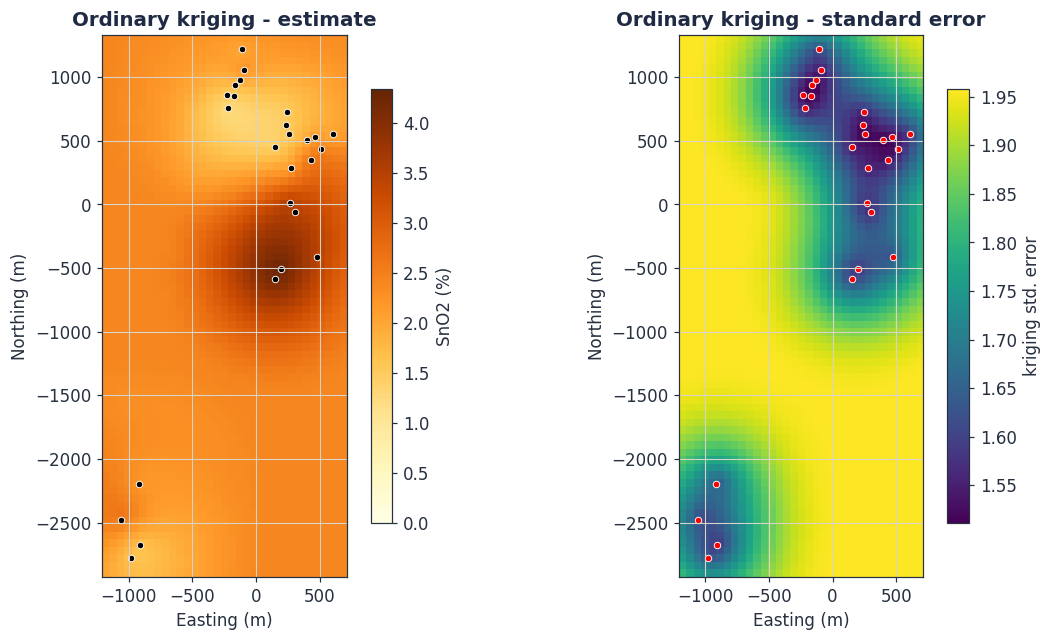
\includegraphics[width=\textwidth]{../assets/figures/fig_kriging.png}
\caption{Toro ordinary kriging. \emph{Left:} grade estimate. \emph{Right:}
kriging standard error from equation (5.8). The standard-error map ---
which no classical estimator can draw --- says exactly where the estimate
can be trusted and drives the classification of Module 6.}
\end{figure}

\begin{torobox}[The Toro cross-validation result]
\begin{center}\small
\begin{tabular}{@{}lrl@{}}
\toprule
\textbf{Metric} & \textbf{Value} & \textbf{Reading}\\
\midrule
Mean error & $+0.02\%$ SnO$_2$ & essentially unbiased --- good\\
RMSE & $1.80\%$ SnO$_2$ & large against a 2.3\% mean grade\\
Correlation est--actual & $0.24$ & weak predictive power\\
\bottomrule
\end{tabular}
\end{center}
The kriging is \emph{unbiased} --- requirement 1 satisfied. But its
\emph{precision is poor}: correlation 0.24 means the estimate barely
out-predicts the global mean. That is not a failure of kriging --- the
BLUE derivation guarantees these are the best linear weights
obtainable. It is a failure of \emph{data}. With a relative nugget of
0.55 and 26 widely spread pits, there is too little spatial signal. The
mathematics has done its job; it has also told you the truth.
\end{torobox}

\begin{keybox}[Why this is the most important result in the course]
A weak cross-validation is not a setback to be hidden --- it is the
estimate quantifying confidence honestly. It is the mathematical proof
that Toro is an Exploration Target. And it is \emph{prescriptive}:
precision will improve only by attacking the nugget (better sampling
protocols, Module 2) and adding data density (drilling). Kriging has
not just estimated the deposit; it has costed and justified the next
exploration budget.
\end{keybox}

\vspace{4pt}{\color{line}\hrule}\vspace{4pt}
{\small\itshape Module 5 of the Toro Resource Estimation course. Next:
Module 6, Block Models, Cut-off Grade and the Resource Statement.}

\end{document}
